\documentclass[conference]{IEEEtran}

\usepackage[T1]{fontenc}
\usepackage[utf8]{inputenc}

\usepackage{amsmath,amssymb,amsfonts}
\usepackage{graphicx}
\usepackage{xcolor}
\usepackage{cite}
\usepackage{url}
\usepackage{booktabs}
\usepackage{listings}
\usepackage{hyperref}

\hypersetup{
    colorlinks=true,
    linkcolor=blue,
    citecolor=blue,
    urlcolor=blue
}

\lstset{
    basicstyle=\ttfamily\scriptsize,
    breaklines=true,
    breakatwhitespace=true,
    postbreak=\mbox{\textcolor{gray}{$\hookrightarrow$}\space},
    columns=fullflexible,
    keepspaces=true,
    showstringspaces=false
}

\lstdefinestyle{yaml}{
    basicstyle=\ttfamily\scriptsize,
    keywordstyle=\color{blue},
    commentstyle=\color{gray},
    stringstyle=\color{teal},
    showstringspaces=false,
    breaklines=true,
    frame=single,
    numbers=left,
    numberstyle=\tiny
}

\begin{document}

\title{HybridHPCScheduler: A Segment-Aware Hybrid Framework for
Constraint-Based and Reinforcement-Learning Scheduling in
Heterogeneous HPC Systems}

\author{\IEEEauthorblockN{Dr. Patrick Lemoine}
\IEEEauthorblockA{
Independent Researcher / HPC and AI Systems Engineer\\
Email: \texttt{lemoine\_patrick@yahoo.ca}\\
ORCID: \href{https://orcid.org/0009-0008-9465-8159}{0009-0008-9465-8159}\\
GitHub: \href{https://github.com/lemoinep/HybridHPCScheduler}
{github.com/lemoinep/HybridHPCScheduler}
}
}

\maketitle

\begin{abstract}
Modern high-performance computing (HPC) systems increasingly combine CPUs,
GPUs, and specialized accelerators such as neural processing units (NPUs),
tensor processing units (TPUs), and data processing units (DPUs). Efficiently
scheduling workloads on such heterogeneous platforms requires reasoning about
device capabilities, memory hierarchies, network links, task dependencies,
resource contention, and execution phases. This paper presents
\textit{HybridHPCScheduler}, an experimental framework for AI-based scheduling
and resource orchestration in heterogeneous HPC environments.

HybridHPCScheduler models workloads as ordered sequences of execution segments
that may be assigned to different device types. The scheduling problem is
formulated as a combinatorial optimization problem and solved either with a
constraint-programming approach based on the CP-SAT solver or with a
reinforcement-learning approach implemented through a custom Gymnasium
environment and a Proximal Policy Optimization (PPO) agent. The framework also
provides topology and accelerator discovery utilities, energy-monitoring
backends, multi-episode benchmarking, result export, visualization, and
configuration comparison tools.

The main contribution of this work is a unified platform combining exact
constraint-based optimization, learning-based adaptive scheduling, and
reproducible experimental evaluation for next-generation heterogeneous HPC
systems. HybridHPCScheduler is currently an evolving research prototype; its
primary objective is to provide a reproducible experimental foundation for
studying hybrid scheduling strategies rather than to serve as a production
exascale resource manager.
\end{abstract}

\begin{IEEEkeywords}
Heterogeneous computing, HPC scheduling, constraint programming, CP-SAT,
reinforcement learning, PPO, GPU scheduling, resource orchestration,
exascale computing, energy-aware computing.
\end{IEEEkeywords}

\section{Introduction}
The growing complexity of scientific computing, artificial intelligence, and
large-scale simulation workloads has made scheduling a central challenge in
modern HPC systems. Contemporary platforms are no longer composed exclusively
of homogeneous CPU nodes. They increasingly integrate GPUs for parallel
numerical computation, NPUs and TPUs for machine-learning inference and
training, and DPUs for offloading networking, storage, and security operations.

In such environments, a single application is rarely executed as one monolithic
task. Instead, it is commonly decomposed into a pipeline of stages: data
ingestion, decoding, preprocessing, inference, fusion, post-processing, and
storage. These stages may have different hardware requirements and may benefit
from execution on different devices. For example, preprocessing may be
CPU-bound, inference may require GPU or NPU acceleration, and data movement may
depend on network bandwidth and latency.

Traditional HPC resource managers, such as Slurm~\cite{slurm}, provide robust
mechanisms for job queuing and resource allocation. However, they are not
always designed to capture fine-grained, segment-level execution behavior
within a job, nor to support rapid experimentation with alternative scheduling
policies. Conversely, learning-based scheduling approaches can adapt to dynamic
workloads, but they require well-defined environments, reproducible benchmarks,
and meaningful evaluation metrics.

\textit{HybridHPCScheduler} addresses these needs by providing an experimental
framework that combines:
\begin{itemize}
    \item a segment-aware model of heterogeneous resources and workloads;
    \item a CP-SAT-based constraint-programming scheduler;
    \item a Gymnasium-based reinforcement-learning environment;
    \item a PPO agent for learning dynamic scheduling policies;
    \item topology and accelerator discovery tools;
    \item energy and thermal monitoring prototypes;
    \item multi-episode benchmarking, visualization, and reporting capabilities.
\end{itemize}

The project is implemented primarily in Python~3.12+ and C++17, with support
for CUDA, MPI, and Slurm-compatible environments. It is currently an evolving
research prototype intended to explore the design space of hybrid scheduling in
heterogeneous HPC systems. In particular, it provides a controlled environment
for comparing constraint-based optimization and reinforcement-learning policies
before their deployment on larger production platforms~\cite{lemoine2026}.

\section{Related Context}
Heterogeneous scheduling differs from conventional job scheduling in several
important ways. First, resources are not interchangeable: a GPU-only task
cannot be executed on a CPU-only device, while a CPU task may be executable on
several device classes with different performance characteristics. Second,
tasks are often organized as directed acyclic graphs (DAGs), where downstream
operations cannot begin until upstream operations have completed. Third,
resource occupancy must be managed carefully to avoid contention on shared
devices, memory subsystems, or communication links.

These characteristics make scheduling decisions more complex than in
homogeneous CPU-only clusters. A scheduler must not only decide when a task can
start, but also determine whether the selected device provides the required
computational capabilities, whether sufficient memory is available, and whether
communication between dependent tasks introduces significant delay.

Constraint programming is well suited to this class of problems because it can
explicitly encode assignment, precedence, capacity, and non-overlap
constraints. The CP-SAT solver provides an effective approach for obtaining
optimal or near-optimal schedules within practical time limits~\cite{cpsat}.

Reinforcement learning offers a complementary perspective. Rather than solving
each scheduling instance from scratch, an RL agent learns a policy that maps
the current system state---such as resource occupancy, ready tasks, and elapsed
time---to scheduling actions. This approach is particularly attractive for
dynamic or recurring workloads, where fast online decisions are
required~\cite{ppo}.

HybridHPCScheduler is designed to support both approaches and to enable their
systematic comparison. By placing constraint-based optimization and
reinforcement learning in a common experimental environment, the framework
allows researchers to evaluate the trade-offs between schedule quality,
decision speed, adaptability, and implementation complexity.

\section{System Overview}
HybridHPCScheduler is structured around four principal components:
\begin{enumerate}
    \item workload and resource modeling;
    \item constraint-based scheduling with CP-SAT;
    \item reinforcement-learning scheduling with Gymnasium and PPO;
    \item benchmarking, visualization, and reporting.
\end{enumerate}

The framework uses YAML configuration files to describe clusters, devices,
memory levels, network links, task pipelines, dependencies, priorities,
deadlines, and reinforcement-learning hyperparameters. This configuration-driven
design makes it possible to define and compare multiple HPC scenarios without
modifying the core scheduler implementation.

This separation of concerns is particularly useful for experimental research.
A user can modify the hardware topology, change the workload structure, or
adjust scheduling parameters while retaining the same scheduling algorithms and
evaluation pipeline. Conversely, new scheduling strategies can be introduced
without rewriting the description of the underlying HPC environment.

\subsection{Heterogeneous Resource Model}
The resource model represents a multi-device computing environment. Devices may
include CPUs, GPUs, NPUs, TPUs, DPUs, and other simulated or real accelerators.

Each device is associated with relevant characteristics such as processing
capability, memory capacity, and connectivity. The framework also models memory
levels attached to devices and network links between resources. Network links
are characterized by concepts such as bandwidth and latency, enabling the
scheduler to reason about communication constraints in addition to computation
time.

Internally, the topology can be represented as a multi-directed graph,
separating three dimensions:
\begin{itemize}
    \item devices;
    \item memory attached to each device;
    \item dependency chains between tasks.
\end{itemize}

Fig.~\ref{fig:model} illustrates the separation between devices, memory
domains, and task-dependency chains in the HybridHPCScheduler resource model.

\begin{figure}[!t]
\centering
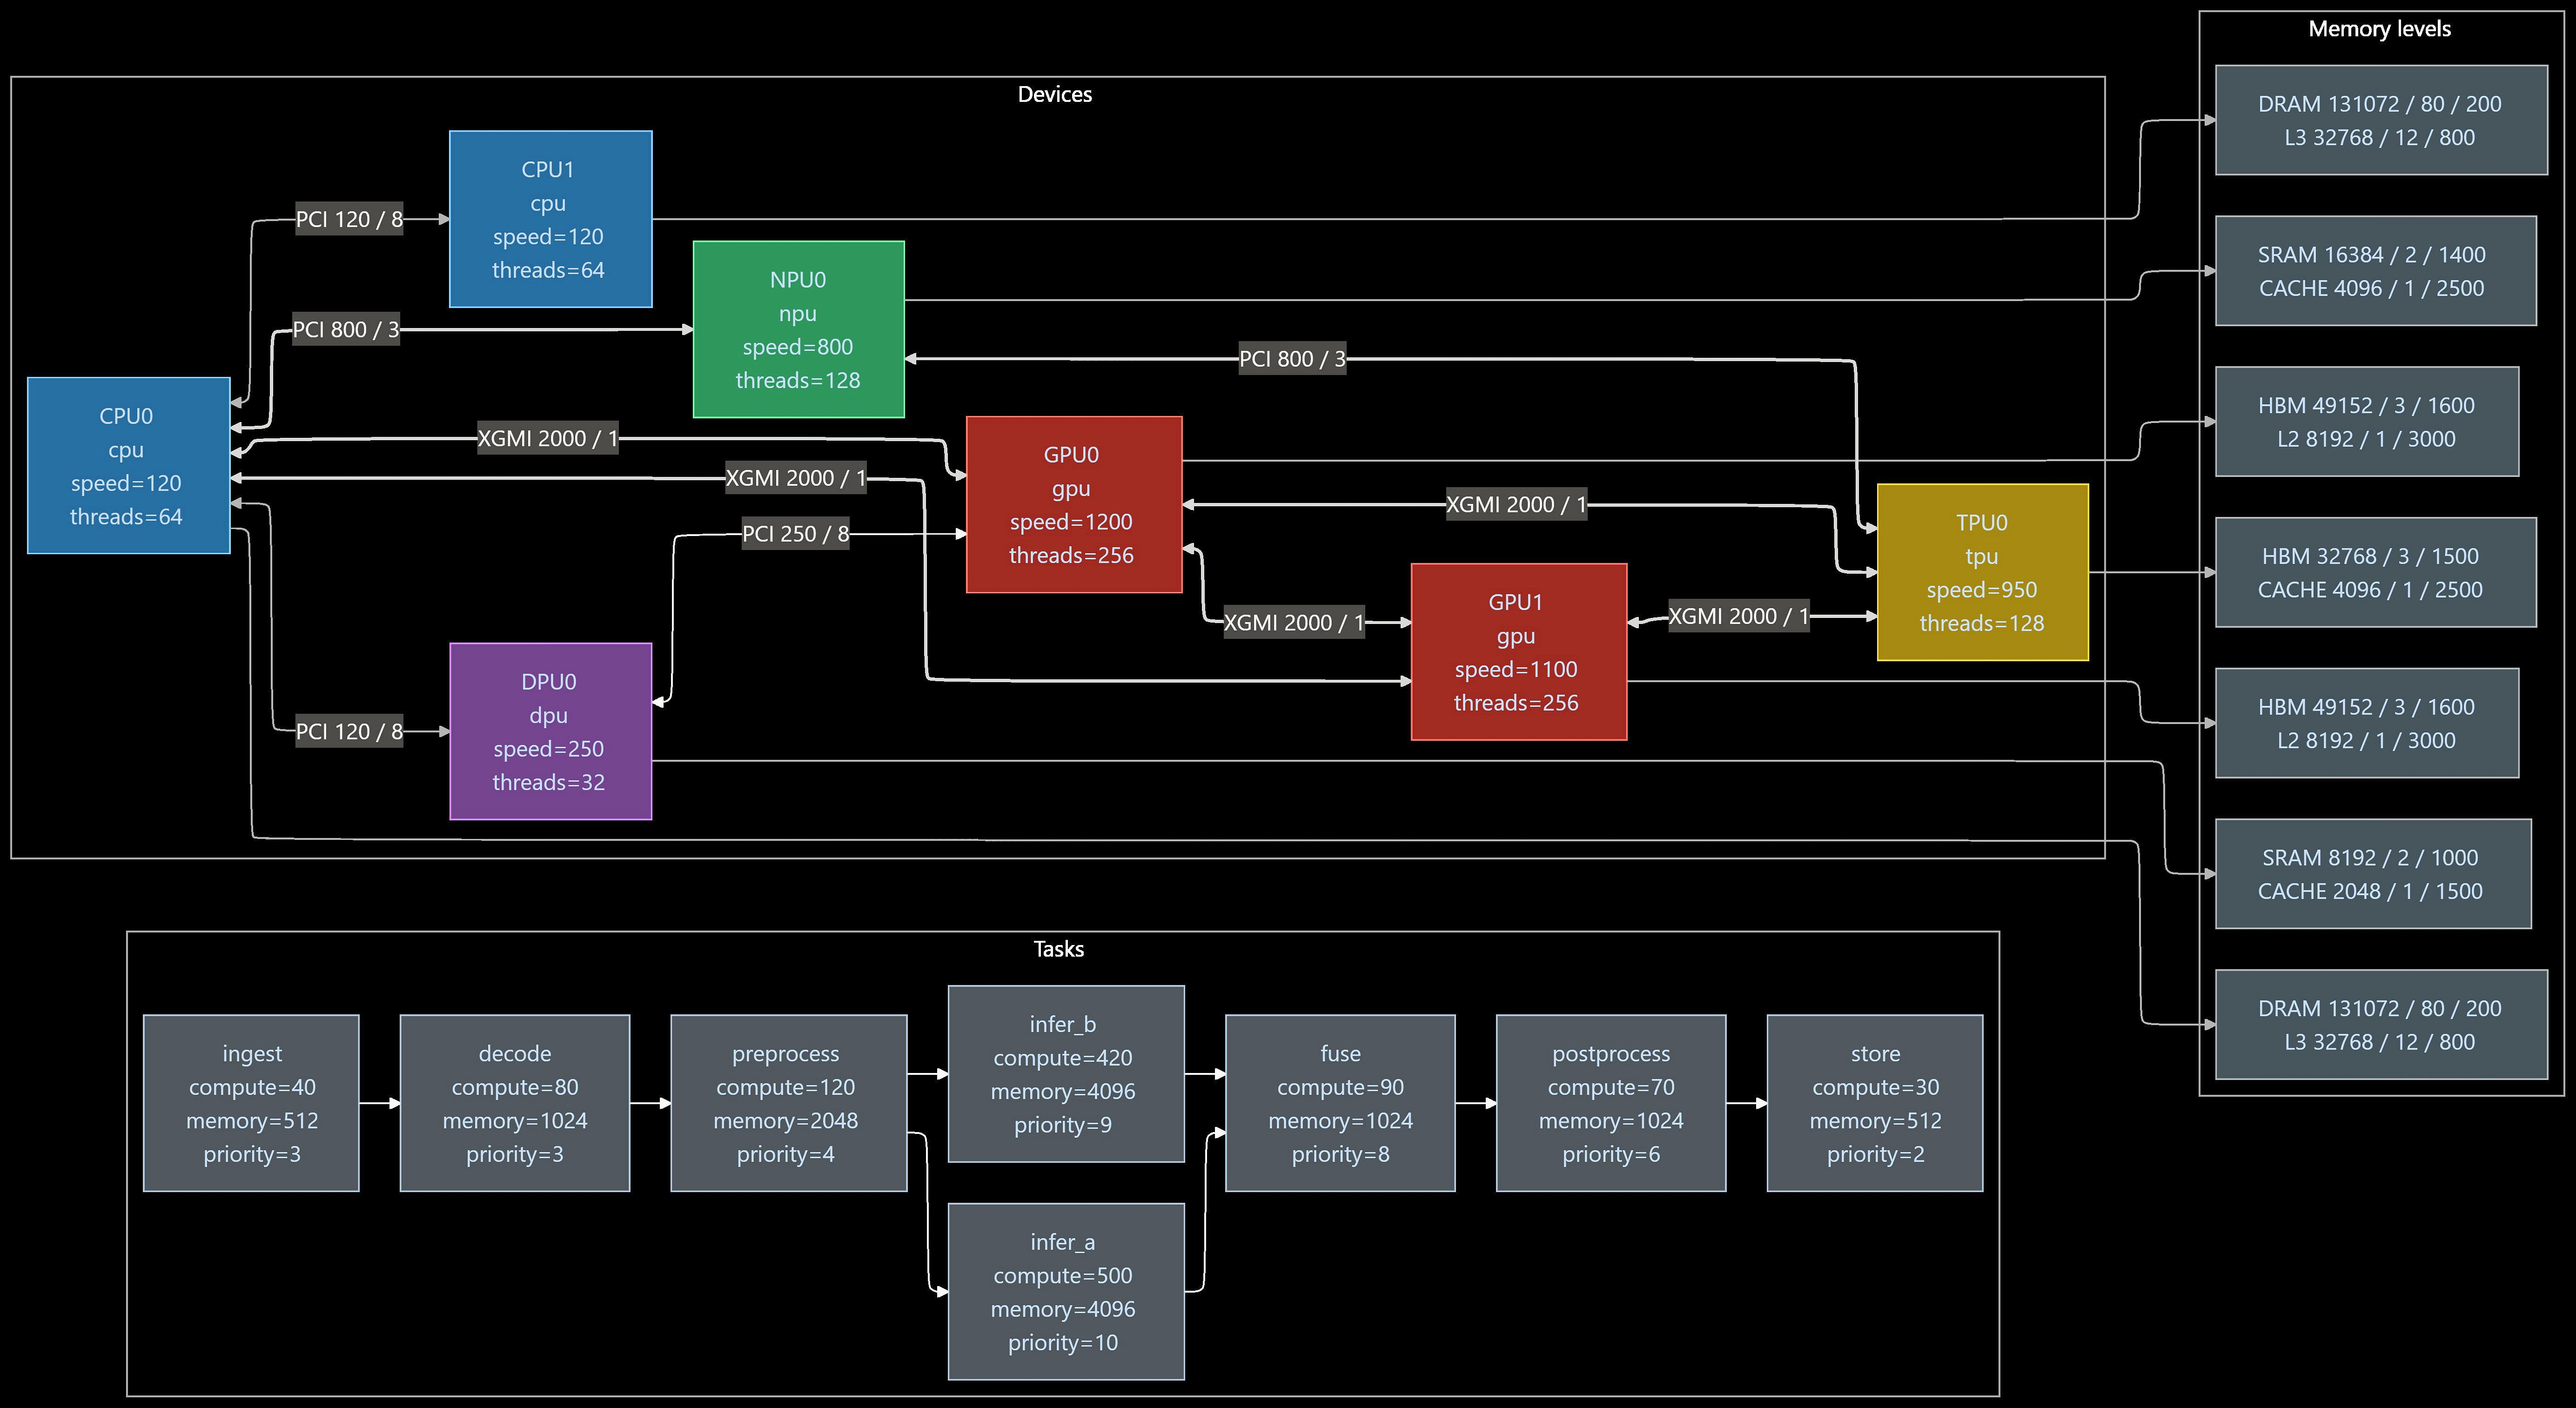
\includegraphics[width=\linewidth]{Images/Model_20260522_000001.jpg}
\caption{Conceptual model of the heterogeneous HPC environment, including
devices, attached memory levels, network links, and task dependencies.}
\label{fig:model}
\end{figure}

This representation supports the analysis of complex HPC environments where
multiple devices, memory domains, and communication paths coexist. It also
allows the scheduler to distinguish between computational constraints, memory
constraints, and communication constraints, which is essential when workloads
involve large data transfers or tightly coupled processing stages.

\subsection{Segment-Aware Workload Model}
HybridHPCScheduler decomposes each job into an ordered set of execution
segments. A segment is a schedulable unit of work that may be assigned to a
particular class of device.

For example, an end-to-end AI pipeline may be modeled as the following ordered
sequence of stages:

\begin{enumerate}
    \item data ingestion;
    \item decoding;
    \item preprocessing;
    \item inference;
    \item fusion;
    \item post-processing;
    \item storage.
\end{enumerate}

In this pipeline, ingestion and storage may execute on CPU-associated
resources, preprocessing may use CPU or GPU resources, while inference may
require a GPU, NPU, or TPU. Each segment may have a different duration
depending on the device to which it is assigned.

This segment-level decomposition is a central feature of the framework. It
allows the scheduler to capture fine-grained execution behavior that would be
hidden if each job were treated as a single indivisible unit. It also enables
more precise resource allocation, since different stages of the same
application can be mapped to the most appropriate hardware resources.

\section{Mathematical Formulation}
\subsection{Problem Setting}
Let:
\begin{itemize}
    \item \(J = \{1,2,\ldots,n\}\) be the set of jobs;
    \item \(S_j = \{1,2,\ldots,m_j\}\) be the ordered set of segments of job
    \(j\);
    \item \(R = \{1,2,\ldots,p\}\) be the set of heterogeneous resources;
    \item \(d_{j,s} > 0\) be the processing time of segment \((j,s)\);
    \item \(R_{j,s} \subseteq R\) be the set of feasible resources for segment
    \((j,s)\).
\end{itemize}

A segment may require a specific device type, have different execution
durations depending on the assigned resource, and be subject to precedence
constraints with other segments.

\subsection{Decision Variables}
For each segment \((j,s)\) and each feasible resource \(r \in R_{j,s}\), the
scheduler defines:
\begin{equation}
x_{j,s,r} \in \{0,1\},
\end{equation}
where \(x_{j,s,r}=1\) if segment \((j,s)\) is assigned to resource \(r\), and
\(0\) otherwise.

The start time and completion time of segment \((j,s)\) are denoted by:
\begin{equation}
t_{j,s} \geq 0,
\end{equation}
\begin{equation}
c_{j,s} = t_{j,s} + d_{j,s}.
\end{equation}

The makespan is defined as:
\begin{equation}
C_{\max} = \max_{j \in J,\; s \in S_j} c_{j,s}.
\end{equation}

To linearize resource-sharing constraints, auxiliary ordering variables may also
be introduced:
\begin{equation}
z_{a,b,r} \in \{0,1\},
\end{equation}
where \(z_{a,b,r}=1\) if segment \(a\) is scheduled before segment \(b\) on
resource \(r\).

\subsection{Objective Function}
The primary scheduling objective is to minimize the makespan:
\begin{equation}
\min C_{\max}.
\end{equation}

The objective can be extended to include additional scheduling criteria, such as
total waiting time, energy consumption, monetary cost, or device-specific
penalties:
\begin{equation}
\min \left[
\alpha C_{\max}
+ \beta \sum_{j=1}^{n} \sum_{s=1}^{m_j} t_{j,s}
+ \gamma \sum_{j=1}^{n} \sum_{s=1}^{m_j}
\sum_{r \in R_{j,s}}
\mathrm{cost}_{j,s,r}\, x_{j,s,r}
\right].
\end{equation}

Here, \(\alpha\), \(\beta\), and \(\gamma\) are user-defined weights. The term
\(\mathrm{cost}_{j,s,r}\) may represent energy cost, monetary cost, or another
resource-specific penalty. This flexible objective allows the scheduler to
balance completion time against other operational concerns, such as energy
efficiency or the cost of using specialized accelerators.

\subsection{Constraints}

\subsubsection{Unique Resource Assignment}
Each segment must be assigned to exactly one feasible resource:
\begin{equation}
\sum_{r \in R_{j,s}} x_{j,s,r} = 1
\quad
\forall j \in J,\; \forall s \in S_j.
\end{equation}

If a segment cannot execute on a given resource, the corresponding assignment
variable is not created or is fixed to zero.

\subsubsection{Precedence Constraints}
Segments belonging to the same job must respect their internal ordering. For
each job \(j\) and each segment \(s < m_j\):
\begin{equation}
t_{j,s+1} \geq c_{j,s}.
\end{equation}

More general dependencies between segments \(u\) and \(v\) are expressed as:
\begin{equation}
t_v \geq c_u
\quad
\text{for each dependency } u \rightarrow v.
\end{equation}

These constraints ensure that a segment cannot begin before all of its
prerequisite segments have completed. They are particularly important for AI
and scientific pipelines, where data produced by an earlier stage is required
by subsequent processing steps.

\subsubsection{Non-Overlap Constraints}
Two segments assigned to the same resource cannot execute simultaneously. For
two distinct segments \(a=(j,s)\) and \(b=(j',s')\), if both are assigned to
resource \(r\), then:
\begin{equation}
t_a + d_a \leq t_b
\end{equation}
or
\begin{equation}
t_b + d_b \leq t_a.
\end{equation}

In the CP-SAT formulation, this disjunction is linearized using ordering
variables:
\begin{equation}
t_a + d_a \leq t_b + M(1-z_{a,b,r}),
\end{equation}
\begin{equation}
t_b + d_b \leq t_a + M z_{a,b,r},
\end{equation}
where \(M\) is a sufficiently large constant.

\subsubsection{Resource Feasibility}
A segment can only be assigned to resources included in its feasible set:
\begin{equation}
x_{j,s,r} = 0
\quad
\forall r \notin R_{j,s}.
\end{equation}

In practice, this constraint is enforced by creating assignment variables only
for feasible resource-segment pairs. This reduces the size of the optimization
model and prevents the scheduler from considering invalid assignments.

\subsubsection{Optional Time-Horizon Constraint}
If required, all segments must complete before a given horizon \(T\):
\begin{equation}
c_{j,s} \leq T
\quad
\forall j \in J,\; \forall s \in S_j.
\end{equation}

This constraint can be used to model deadlines, service-level objectives, or
time-limited experimental scenarios.

\subsection{Compact Formulation}
The complete scheduling problem can be summarized as:
\begin{equation}
\begin{aligned}
\min \quad & C_{\max} \\
\text{s.t.} \quad
& \sum_{r \in R_{j,s}} x_{j,s,r} = 1
&& \forall j,s \\
& t_{j,s+1} \geq c_{j,s}
&& \forall j,\; s < |S_j| \\
& c_{j,s} = t_{j,s} + d_{j,s}
&& \forall j,s \\
& C_{\max} \geq c_{j,s}
&& \forall j,s \\
& t_a + d_a \leq t_b \;\lor\; t_b + d_b \leq t_a
&& \forall a,b \in r \\
& x_{j,s,r} \in \{0,1\},\; t_{j,s} \geq 0
&& \forall j,s,r.
\end{aligned}
\end{equation}

The non-overlap constraint applies to every pair of segments \(a\) and \(b\)
assigned to the same resource \(r\). This formulation defines a combinatorial
optimization problem over a heterogeneous, segment-aware resource model.

\section{Constraint-Based Scheduling With CP-SAT}
The first scheduling approach implemented in HybridHPCScheduler encodes the
problem as a constraint-programming model solved with CP-SAT.

The CP-SAT formulation explicitly represents:
\begin{itemize}
    \item segment-to-resource assignment;
    \item task and segment precedence;
    \item resource capacity and non-overlap;
    \item device feasibility;
    \item optional deadlines and scheduling horizons;
    \item optional cost, energy, or priority terms.
\end{itemize}

Given a workload description and a cluster configuration, CP-SAT searches for
an optimal or near-optimal schedule. This approach is particularly useful when
the scheduling constraints are complex and when solution quality is more
important than immediate decision speed.

Because the model is expressed explicitly, CP-SAT can also serve as a reference
method for evaluating learned scheduling policies. For example, the makespan
produced by a reinforcement-learning agent can be compared with the best
schedule found by CP-SAT under the same workload and resource constraints.

\section{Reinforcement-Learning Scheduling}
\subsection{Markov Decision Process Formulation}
HybridHPCScheduler also models scheduling as a Markov Decision Process (MDP).
A custom Gymnasium environment~\cite{gymnasium} formalizes the interaction
between the scheduler and the HPC system.

The main elements of the MDP are:
\begin{itemize}
    \item \textbf{State:} current resource occupancy, ready segments, pending
    dependencies, elapsed time, and other workload or topology features;
    \item \textbf{Action:} assignment and ordering decisions for available
    segments;
    \item \textbf{Reward:} typically related to minimizing makespan, lateness,
    congestion, or a weighted combination of performance metrics;
    \item \textbf{Transition:} the evolution of the system after a scheduling
    decision, including task completion, resource release, and the activation
    of dependent segments.
\end{itemize}

This formulation enables the scheduler to learn policies that adapt to workload
variability and changing system conditions. Unlike a static optimization
approach, the learned policy can potentially make rapid decisions when new
tasks arrive or when resource availability changes.

\subsection{PPO Agent}
The framework integrates a Proximal Policy Optimization (PPO) agent to learn
scheduling policies through multi-episode training. PPO is a policy-gradient
reinforcement-learning algorithm that improves policy stability by limiting the
magnitude of policy updates during training~\cite{ppo}.

In HybridHPCScheduler, the PPO agent observes the state of the scheduling
environment and selects actions that determine how ready segments are assigned
to resources. Through repeated episodes, the agent learns to balance competing
objectives such as reducing makespan, avoiding resource contention, respecting
dependencies, and handling heterogeneous device constraints.

The learned policy can then be benchmarked against the CP-SAT scheduler or
against other heuristic and learning-based strategies. This comparison helps
identify situations in which learned policies provide a practical advantage,
for example when scheduling decisions must be made frequently or when the
workload exhibits recurring patterns.

\section{Benchmarking and Experimental Workflow}
HybridHPCScheduler includes a comprehensive experimental workflow designed to
support reproducible evaluation. The workflow covers agent training,
multi-episode benchmarking, detailed execution analysis, visualization, and
comparison across multiple cluster configurations.

\subsection{Training}
A PPO agent can be trained on a specified HPC configuration using:
\begin{lstlisting}[language=bash]
python main.py train \
    --config configs/<your_config>.yaml \
    --output <output_dir>
\end{lstlisting}

The configuration file defines the cluster, devices, tasks, dependencies,
topology, and reinforcement-learning hyperparameters. The output directory
contains the trained model and training logs.

\subsection{Benchmarking}
A trained agent can be evaluated over multiple episodes using:
\begin{lstlisting}[language=bash]
python main.py benchmark \
    --config configs/<your_config>.yaml \
    --episodes <n_episodes> \
    --output <output_dir>
\end{lstlisting}

The benchmarking pipeline produces summary statistics, including files such as
\texttt{benchmark\_summary.csv} and \texttt{benchmark\_stats.csv}. These files
can be used to compare the average and variability of scheduling performance
across independent evaluation episodes.

\subsection{Detailed Evaluation}
For detailed analysis, the framework supports evaluation runs that export
execution traces and per-step metrics:
\begin{lstlisting}[language=bash]
python main.py evaluate \
    --config configs/<your_config>.yaml \
    --output <output_dir>
\end{lstlisting}

This mode is useful for inspecting individual scheduling decisions, resource
utilization, task waiting times, and constraint violations. It can also help
identify pathological cases in which an agent repeatedly selects inefficient
assignments or fails to exploit available accelerators.

\subsection{Visualization and Reporting}
The framework can generate plots and reports from saved results:
\begin{lstlisting}[language=bash]
python main.py plot \
    --config configs/<your_config>.yaml \
    --output <output_dir>
\end{lstlisting}

It also supports Gantt-chart and timeline visualization:
\begin{lstlisting}[language=bash]
python main.py visualize \
    --config configs/<your_config>.yaml \
    --output <output_dir>
\end{lstlisting}

Batch visualization across multiple runs is available through:
\begin{lstlisting}[language=bash]
python main.py visualize-all \
    --output <output_root_dir>
\end{lstlisting}

Results can be exported in several formats:
\begin{itemize}
    \item CSV for numerical analysis;
    \item PNG for visualization;
    \item JSONL for structured logging and reproducibility;
    \item HTML for interactive or report-oriented outputs.
\end{itemize}

\subsection{Configuration Comparison}
Multiple HPC configurations can be compared side by side:
\begin{lstlisting}[language=bash]
python main.py compare \
    --configs configs/config1.yaml configs/config2.yaml \
    --output <output_dir>
\end{lstlisting}

This command generates aggregated statistics and comparison plots across
configurations, enabling systematic evaluation of different cluster topologies,
workload structures, and scheduling policies. Such comparisons are particularly
useful for studying how changes in device count, memory capacity, or network
connectivity affect scheduling behavior.

\section{Topology and Accelerator Discovery}
To support realistic experimentation, HybridHPCScheduler includes C++ utilities
for discovering hardware topology and accelerators on Linux systems. These
tools help bridge the gap between abstract scheduling models and the actual
hardware characteristics of HPC nodes.

\subsection{ScanExascaleForLinux}
\texttt{ScanExascaleForLinux.cpp} is an exascale workload and topology
generator. It uses hwloc~\cite{hwloc} to probe node topology and detect real
CPUs and GPUs. It can also discover NPUs, TPUs, and DPUs through
\texttt{sysfs}.

The tool combines detected hardware with configurable simulated accelerators to
construct a synthetic exascale node model. It generates a YAML file, by default
named \texttt{ScanExascale.yaml}, describing:
\begin{itemize}
    \item devices;
    \item interconnect topology;
    \item an end-to-end AI pipeline DAG;
    \item task priorities;
    \item deadlines.
\end{itemize}

The generated YAML file can then be used as input to the hybrid scheduler for
benchmarking scheduling policies across heterogeneous CPUs, GPUs, NPUs, TPUs,
and DPUs.

The following commands illustrate how to generate a topology description and
configure the resulting synthetic node model:

\begin{lstlisting}[language=bash]
./ScanExascaleForLinux --verbose
./ScanExascaleForLinux --output=MyNode.yaml
./ScanExascaleForLinux --real --no-sim-gpu --no-real-accels
./ScanExascaleForLinux \
    --node-type=ai_node \
    --cluster-desc=ClusterDescription.yaml
\end{lstlisting}

\subsection{Accelerator Detection}
\texttt{ScanExascaleReportAccelNTDu.cpp} detects AI and network accelerators,
including NPUs, TPUs, and DPUs. The utility traverses PCI and USB buses through
\texttt{sysfs}, uses the system \texttt{pci.ids} and \texttt{usb.ids}
databases, and classifies devices using identifiers, drivers, class codes, and
textual fingerprints.

It can generate:
\begin{itemize}
    \item a human-readable accelerator summary;
    \item a structured JSON inventory;
    \item a CSV file containing decoded device-identification fields.
\end{itemize}

The following commands illustrate how to run the detector and export its
results in different formats:

\begin{lstlisting}[language=bash]
./ScanExascaleReportAccelNTDu
./ScanExascaleReportAccelNTDu --verbose
./ScanExascaleReportAccelNTDu --json
./ScanExascaleReportAccelNTDu --csv accelerators.csv
\end{lstlisting}

These tools provide a practical bridge between real hardware discovery and
scheduler-level experimentation. They allow generated configurations to reflect
the actual devices available on a node while still supporting controlled
synthetic extensions for benchmarking.

\section{Energy Monitoring and Thermal Visualization}
Energy consumption and thermal behavior are increasingly important in
large-scale HPC systems. HybridHPCScheduler includes a prototype for energy
monitoring and heat-map visualization. This capability is intended to support
future scheduling policies that consider not only performance but also power
consumption and thermal constraints.

\subsection{CPU Power Backends}
The project provides several CPU power-monitoring backends:
\begin{itemize}
    \item \texttt{read\_rapl\_packages\_intel.cpp}: reads Intel
    RAPL~\cite{rapl} model-specific registers (MSRs) on Linux to estimate
    per-package CPU power;
    \item \texttt{read\_rapl\_packages\_amd\_stub.cpp}: an AMD stub backend that
    generates simulated per-package power values;
    \item \texttt{read\_rapl\_packages\_amd\_real.cpp}: an AMD backend that uses
    \texttt{perf stat -a -e power/energy-pkg/} over a short interval to
    estimate total energy and derive average power per package.
\end{itemize}

The Intel backend outputs data in the following CSV format:
\begin{lstlisting}[language=bash]
package_id,power_watts
\end{lstlisting}

\subsection{Energy Map Generation}
The Python utility \texttt{energy\_map.py} loads an energy configuration file,
invokes the appropriate CPU backend, and uses NVIDIA NVML~\cite{nvml} for GPU
metrics. It produces:
\begin{itemize}
    \item \texttt{device\_metrics.csv};
    \item \texttt{energy\_map\_power.png};
    \item \texttt{energy\_map\_temperature.png}.
\end{itemize}

A simulated example is:
\begin{lstlisting}[language=bash]
python energy_map.py \
    --energy-config configs/energy.yaml \
    --output outputs/energy_demo \
    --mode simulated
\end{lstlisting}

When hardware backends are available, real measurements can be collected using:
\begin{lstlisting}[language=bash]
python energy_map.py \
    --energy-config configs/energy.yaml \
    --topology configs/scan_exascale_hwloc.yaml \
    --output outputs/energy_real \
    --mode real
\end{lstlisting}

This capability provides a foundation for future energy-aware and thermal-aware
scheduling policies. For example, the scheduler could avoid placing additional
work on devices that are already operating close to a power or temperature
limit.

\section{Case Study: Heterogeneous AI Pipeline Scheduling}
A representative use case for HybridHPCScheduler is the scheduling of an
end-to-end AI inference pipeline on a heterogeneous node.

The pipeline consists of the following stages:
\begin{enumerate}
    \item data ingestion;
    \item decoding;
    \item preprocessing;
    \item inference;
    \item fusion;
    \item post-processing;
    \item storage.
\end{enumerate}

Each stage is modeled as a segment with its own feasible device set, duration,
priority, and deadline. The scheduler must determine:
\begin{itemize}
    \item which device executes each segment;
    \item when each segment starts;
    \item how precedence constraints are respected;
    \item how contention on shared resources is avoided;
    \item whether deadlines can be satisfied;
    \item how the overall makespan can be reduced.
\end{itemize}

The CP-SAT formulation can compute a high-quality schedule for a given
instance, while the PPO agent can learn a reusable policy for similar workloads.
Comparing both approaches provides insight into the trade-off between exact
optimization quality and learned-policy inference speed.

This case study also highlights the importance of segment-level scheduling. A
global scheduler that treats the entire pipeline as one job may miss
opportunities to overlap independent stages or to assign individual stages to
the most appropriate accelerators.

\section{Discussion}
HybridHPCScheduler illustrates the complementarity of constraint-based
optimization and reinforcement learning. Table~\ref{tab:comparison} summarizes
the principal differences, strengths, limitations, and appropriate use cases of
the two scheduling approaches.

\begin{table}[!t]
\caption{Complementarity of CP-SAT and PPO-Based Scheduling Approaches}
\label{tab:comparison}
\centering
\begin{tabular}{p{0.16\linewidth}p{0.34\linewidth}p{0.34\linewidth}}
\toprule
\textbf{Aspect} & \textbf{CP-SAT Scheduling} & \textbf{PPO-Based Scheduling} \\
\midrule
Decision paradigm & Exact or near-exact optimization & Learned approximate policy \\
\addlinespace
Strengths & Handles complex constraints explicitly; provides high-quality schedules & Fast inference after training; adaptable to dynamic workloads \\
\addlinespace
Limitations & May become computationally expensive for large instances & Requires training data, reward design, and generalization validation \\
\addlinespace
Best suited for & Offline planning, benchmarking, reference schedules & Online or recurring scheduling scenarios \\
\addlinespace
Output & Optimized schedule & Scheduling policy \\
\bottomrule
\end{tabular}
\end{table}

The framework does not treat these approaches as mutually exclusive. Instead, it
enables their coexistence within a common workload, topology, and evaluation
model. This design supports future hybrid strategies, for example using CP-SAT
to generate high-quality training demonstrations or using reinforcement
learning to warm-start constraint-based optimization.

Overall, Table~\ref{tab:comparison} suggests that CP-SAT and PPO-based
scheduling are best viewed as complementary components of a broader scheduling
architecture rather than as competing alternatives.

\section{Future Work}
Several directions are planned for the continued development of
HybridHPCScheduler:
\begin{itemize}
    \item development of a 3D visualization interface for navigating complex
    HPC environments;
    \item deeper integration with Slurm and real cluster resource managers;
    \item more extensive energy-aware and thermal-aware scheduling policies;
    \item multi-objective optimization incorporating makespan, energy, cost,
    fairness, and deadline violations;
    \item larger-scale benchmarking on realistic exascale-inspired topologies;
    \item improved generalization of PPO policies across heterogeneous workloads
    and cluster configurations;
    \item hybrid CP-SAT/RL methods, including imitation learning from optimized
    schedules and learned heuristics for guiding constraint solving.
\end{itemize}

\section{Conclusion}
This paper presented \textit{HybridHPCScheduler}, an experimental framework for
intelligent scheduling in heterogeneous HPC environments. The system introduces
a segment-aware scheduling model capable of representing fine-grained execution
stages across CPUs, GPUs, and specialized accelerators.

The framework combines a CP-SAT-based constraint-programming scheduler with a
Gymnasium-based reinforcement-learning environment and a PPO agent. It further
provides topology discovery, accelerator detection, energy monitoring,
benchmarking, visualization, and reproducible result-export capabilities.

By unifying constraint-based optimization and learning-based scheduling in a
common experimental platform, HybridHPCScheduler provides a practical foundation
for studying next-generation scheduling challenges in heterogeneous and
exascale-oriented HPC systems.

\section*{Acknowledgment}
The author acknowledges the open-source software ecosystem that supports this
work, including Python, PyTorch, Gymnasium, Google OR-Tools, hwloc, Linux
perf, and NVIDIA NVML.

\begin{thebibliography}{10}

\bibitem{lemoine2026}
P. Lemoine, ``HybridHPCScheduler: Hybrid HPC Scheduler,'' GitHub repository,
2026. [Online]. Available:
\url{https://github.com/lemoinep/HybridHPCScheduler}

\bibitem{cpsat}
L. Perron and F. Didier, ``CP-SAT,'' Google OR-Tools. [Online]. Available:
\url{https://developers.google.com/optimization/cp/cp_solver}

\bibitem{ppo}
J. Schulman, F. Wolski, P. Dhariwal, A. Radford, and O. Klimov, ``Proximal
Policy Optimization Algorithms,'' \textit{arXiv preprint arXiv:1707.06347},
2017.

\bibitem{gymnasium}
M. Towers et al., ``Gymnasium: A Standard Interface for Reinforcement Learning
Environments,'' \textit{arXiv preprint arXiv:2407.17032}, 2024.

\bibitem{slurm}
A. B. Yoo, M. A. Jette, and M. Grondona, ``SLURM: Simple Linux Utility for
Resource Management,'' in \textit{Job Scheduling Strategies for Parallel
Processing}, Springer, 2003.

\bibitem{topcuoglu}
H. Topcuoglu, S. Hariri, and M.-Y. Wu, ``Performance-Effective and
Low-Complexity Task Scheduling for Heterogeneous Computing,''
\textit{IEEE Transactions on Parallel and Distributed Systems}, vol. 13, no. 3,
pp. 260--274, 2002.

\bibitem{hwloc}
F. Broquedis et al., ``hwloc: A Generic Framework for Managing Hardware
Affinities in HPC Applications,'' in \textit{Proc. 18th Euromicro International
Conference on Parallel, Distributed and Network-Based Processing}, 2010.

\bibitem{rapl}
Intel Corporation, ``Running Average Power Limit (RAPL) Energy Exposed
Interface,'' Linux kernel documentation. [Online]. Available:
\url{https://docs.kernel.org/power/runtime_pm.html}

\bibitem{nvml}
NVIDIA Corporation, ``NVIDIA Management Library (NVML).'' [Online]. Available:
\url{https://developer.nvidia.com/nvidia-management-library-nvml}

\end{thebibliography}

\end{document}